\PassOptionsToPackage{no-math,cm-default}{fontspec}
\documentclass[twoside,nofonts,internet,shmeiwseis]{thewria}
\usepackage{amsmath}
\usepackage{xgreek}
\let\hbar\relax
\defaultfontfeatures{Mapping=tex-text,Scale=MatchLowercase}
\setmainfont[Mapping=tex-text,Numbers=Lining,Scale=1.0,BoldFont={Minion Pro Bold}]{Minion Pro}
\newfontfamily\scfont{GFS Artemisia}
\font\icon = "Webdings"
\usepackage[amsbb]{mtpro2}
\usepackage{tikz,pgfplots}
\tkzSetUpPoint[size=7,fill=white]
\xroma{red!70!black}


\newlist{rlist}{enumerate}{3}
\setlist[rlist]{itemsep=0mm,label=\textcolor{\xrwma}{\roman*.}}
\newlist{brlist}{enumerate}{3}
\setlist[brlist]{itemsep=0mm,label=\bf\roman*.}
\newlist{tropos}{enumerate}{3}
\setlist[tropos]{label=\bf\textit{\arabic*\textsuperscript{oς}\;Τρόπος :},leftmargin=0cm,itemindent=2.3cm,ref=\bf{\arabic*\textsuperscript{oς}\;Τρόπος}}
\newcommand{\tss}[1]{\textsuperscript{#1}}
\newcommand{\tssL}[1]{\MakeLowercase{\textsuperscript{#1}}}

\usepackage{hhline}
\usepackage{gensymb}
\setlist[enumerate]{label=\bf{\large{\textcolor{\xrwma}{\arabic*.}}}}
\usepackage{multicol}
\usepackage{wrap-rl}
\usepackage{mathimatika}

\begin{document}
\titlos{ΜΑΘΗΜΑΤΙΚΑ ΚΑΤΕΥΘΥΝΣΗΣ Β΄ ΛΥΚΕΙΟΥ}{ΔΙΑΝΥΣΜΑΤΑ}{Η έννοια του διανύσματος}
\orismoi
\Orismos{Διανυσματικό μέγεθοσ}
Διανυσματικό ονομάζεται ενα μέγεθος το οποίο προσδιορίζεται από το μέτρο του αλλά και τη διεύθυνση και τη φορά του.\\\\
\Orismos{Διανυσμα}
Διάνυσμα ονομάζεται ένα προσανατολισμένο ευθύγραμμο τμήμα, δηλαδή ένα ευθύγραμμο τμήμα το οποίο έχει μια συγκεκριμένη κατεύθυνση.
\begin{itemize}
\wrapr{-13mm}{8}{4cm}{0mm}{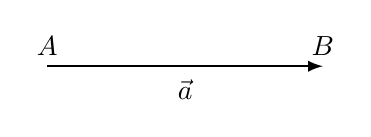
\begin{tikzpicture}
\draw[-latex,line width=.3mm] (0,1) node[anchor=south] (A){$A
$}--(3.5,1) node[anchor=south] (B){$B
$};
\node(a) at (1.75,.7){$ \vec{a} $};
\tkzDrawPoint[size=7,fill=black](0,1)
\end{tikzpicture}}{
\item Τα στοιχεία ενός διανύσματος είναι η φορά, η διεύθυνση και το μέτρο.
\item Η διεύθυνση μαζί με τη φορά ορίζουν την \textbf{κατεύθυνση} του διανύσματος.}
\item Τα άκρα ενός διανύσματος ονομάζονται \textbf{αρχή} (Α) και \textbf{πέρας} (Β). Κάθε διάνυσμα συμβολίζεται με το όνομα του ευθύγραμμου τμήματος που ορίζουν τα άκρα του : $  \overrightarrow{AB}$ ή με ένα μικρό γράμμα : $ \vec{a} $.
\item Το μέτρο του διανύσματος είναι το μήκος του ευθύγραμμου τμήματος $ ΑΒ $.
\item Το διάνυσμα του οποίου τα άκρα ταυτίζονται ονομάζεται \textbf{μηδενικό διάνυσμα} και συμβολίζεται με $ \vec{0} : \overrightarrow{AA}=\vec{0}$.
\end{itemize}
\Orismos{Φορέασ - Διεύθυνση και φορά διανυσματοσ}
Φορέας ενός διανύσματος ονομάζεται η ευθεία στην οποία βρίσκεται πάνω το διάνυσμα. Ο φορέας ενός διανύσματος καθορίζει τη διεύθυνση του. 
\begin{center}
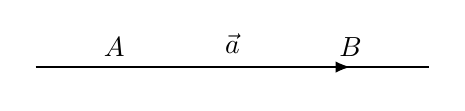
\begin{tikzpicture}
\clip (-1.1,-.2) rectangle (4.1,.5);
\draw (-1,0) -- (4,0);
\draw[-latex,line width=.3mm] (0,0) node[anchor=south] (A){$A
$}--(3,0) node[anchor=south] (B){$B
$} ;
\node(a) at (1.5,.3){$ \vec{a} $};
\tkzDrawPoint[size=7,fill=black](0,0)
\end{tikzpicture}
\end{center}
Η φορά του διανύσματος μας δίνει τον προσανατολισμό του πάνω στον φορέα, δηλαδή τη διάταξη των άκρων του πάνω στο φορέα. Μας δείχνει προς ποιό μέρος \textquotedblleft κινείται\textquotedblright\; το διάνυσμα πάνω στη ευθεία.\\\\
\Orismos{Παράλληλα - Συγγραμμικά διανύσματα}
Παράλληλα ή συγγραμμικά διανύσματα ονομάζονται τα διανύσματα τα οποία έχουν κοινό φορέα ή παράλληλους φορείς. Τα παράλληλα διανύσματα έχουν την ίδια διεύθυνση.
\begin{center}
\begin{tabular}{ccc}
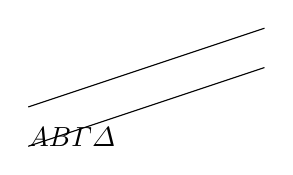
\begin{tikzpicture}
\draw (0,0)--(3,1);
\draw (0,0.5)--(3,1.5);
\dianysma{1,.333}{2.4,.8}{A}{B}
\dianysma{1.8,1.1}{.6,.7}{C}{D}
\tkzLabelPoint[below](A){$A$}
\tkzLabelPoint[below](B){$B$}
\tkzLabelPoint[above](C){$\varGamma$}
\tkzLabelPoint[above](D){$\varDelta$}
\end{tikzpicture}
	&  & 
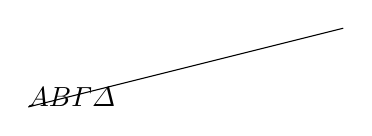
\begin{tikzpicture}
\draw (0,0)--(4,1);
\dianysma{.4,.1}{1.6,.4}{A}{B}
\dianysma{3.6,.9}{2,.5}{C}{D}
\tkzDefPoint(0,-.5){E}
\tkzLabelPoint[below](A){$A$}
\tkzLabelPoint[below](B){$B$}
\tkzLabelPoint[above](C){$\varGamma$}
\tkzLabelPoint[above](D){$\varDelta$}
\end{tikzpicture}
\end{tabular} 
\end{center}
\Orismos{Ομμόροπα - Αντίρροπα διανύσματα}
\begin{enumerate}[itemsep=0mm]
\vspace{-5mm}
\item \textbf{Ομόρροπα}\\Τα διανύσματα που έχουν ίδια διεύθυνση και ίδια φορά λέγονται ομόρροπα. Είναι παράλληλα και η ευθεία που διέρχεται από τις αρχές τους τα αφήνει στο ίδιο ημιεπίπεδο. Ανάμεσα σε δύο ομόρροπα διανύσματα χρησιμοποιούμε το συμβολισμό $ \upuparrows $. Τα ομόρροπα διανύσματα έχουν την ίδια κατεύθυνση.
\begin{itemize}[itemsep=0mm]
\item Ανάμεσα σε δύο ομόρροπα διανύσματα χρησιμοποιούμε το συμβολισμό $ \upuparrows $.
\item Τα ομόρροπα διανύσματα έχουν την ίδια κατεύθυνση.
\end{itemize}
\begin{center}
\begin{tabular}{ccc}
\begin{tikzpicture}[scale=0.7,y=0.7cm]
\dianysma{-3,-0.5}{0,0.5}{A}{B}
\dianysma{-3.5,-2}{-0.5,-1}{C}{D}
\draw[dashed] (-2.5,1) -- (-4,-3.5);
\node at (-3.3,-0.4) {$A$};
\node at (0.2,0.6) {$B$};
\node at (-3.8,-2) {$\varGamma$};
\node at (-0.2,-0.8) {$\varDelta$};
\node at (-2,-4) {$\overrightarrow{AB}\upuparrows\overrightarrow{\varGamma\varDelta}$};
\end{tikzpicture}	&  & \begin{tikzpicture}[scale=0.7,y=0.7cm]
\dianysma{-3,-0.5}{0,0.5}{A}{B}
\dianysma{-3.5,-2}{-6.5,-3}{C}{D}
\draw[dashed] (-2.5,1) -- (-4,-3.5);
\node at (-3.3,-0.4) {$A$};
\node at (0.2,0.6) {$B$};
\node at (-3.8,-1.7) {$\varGamma$};
\node at (-6.8,-3) {$\varDelta$};
\node at (-2,-4) {$\overrightarrow{AB}\updownarrows\overrightarrow{\varGamma\varDelta}$};
\end{tikzpicture} \\ 
\end{tabular} 
\end{center}
\item \textbf{Αντίρροπα}\\
Τα διανύσματα που έχουν ίδια διεύθυνση και ίδια φορά λέγονται αντίρροπα. Είναι παράλληλα και βρίσκονται εκατέρωθεν της ευθείας που διέρχεται από τις αρχές τους. 
\begin{itemize}[itemsep=0mm]
\item Ανάμεσα σε δύο αντίρροπα διανύσματα χρησιμοποιούμε το συμβολισμό $ \updownarrows $.
\item Τα αντίρροπα διανύσματα έχουν αντίθετες κατευθύνσεις.
\end{itemize}
\end{enumerate}
\Orismos{Ίσα - Αντίθετα διανύσματα}
\vspace{-5mm}
\begin{enumerate}[itemsep=0mm]
\item \textbf{Ίσα διανύσματα}\\
Ίσα λεγονται τα ομόρροπα διανύσματα που έχουν ίσα μέτρα.
\item \textbf{Αντίθετα διανύσματα}\\
Αντίθετα λεγονται τα αντίρροπα διανύσματα που έχουν ίσα μέτρα.
\end{enumerate}
\Orismos{Γωνία διανυσμάτων}
Γωνία δύο μη μηδενικών διανυσμάτων $ \overrightarrow{OA}=\vec{a} $ και $ \overrightarrow{OB}=\vec{\beta} $ ονομάζεται η κυρτή γωνία που σχηματίζουν οι φορείς των δύο διανυσμάτων.
\begin{itemize}[itemsep=0mm]
\item Η γωνία των διανυσμάτων $ \vec{a} $ και $ \vec{\beta} $ συμβολίζεται με $ \gwndian{a}{\beta} $.
\item Η γωνία $ \theta $ δύο διανυσμάτων παίρνει τιμές από $ 0\degree $ μέχρι $ 180\degree $ : $ 0\degree\leq\theta\leq 180\degree $ ή $ 0\leq\theta\leq \pi $.
\item Αν $ \theta=0 $ τότε τα διανύσματα $ \vec{a} $ και $ \vec{\beta} $ είναι ομόρροπα : $ \theta=0\Rightarrow \vec{a}\upuparrows \vec{\beta} $.
\item Αν $ \theta=\pi $ τότε τα διανύσματα $ \vec{a} $ και $ \vec{\beta} $ είναι αντίρροπα : $ \theta=\pi\Rightarrow \vec{a}\updownarrows \vec{\beta} $.
\item Αν $ \theta=\frac{\pi}{2} $ τότε τα διανύσματα $ \vec{a} $ και $ \vec{\beta} $ είναι κάθετα : $ \theta=\frac{\pi}{2}\Rightarrow \vec{a}\bot \vec{\beta} $.
\end{itemize}
\end{document}
